\documentclass{article}

\usepackage{graphicx}
\usepackage{tikz}
\usepackage{tikzsymbols}
\usetikzlibrary{calc,patterns,shapes.geometric}
\pagestyle{empty}
\usepackage[margin=0pt]{geometry}
\geometry{papersize={14in,12in}}

\def\centerarc[#1](#2)(#3:#4:#5){\draw[#1] ($(#2)+({#5*cos(#3)},{#5*sin(#3)})$) arc (#3:#4:#5);}

\begin{document}
	\begin{figure}
		\centering
		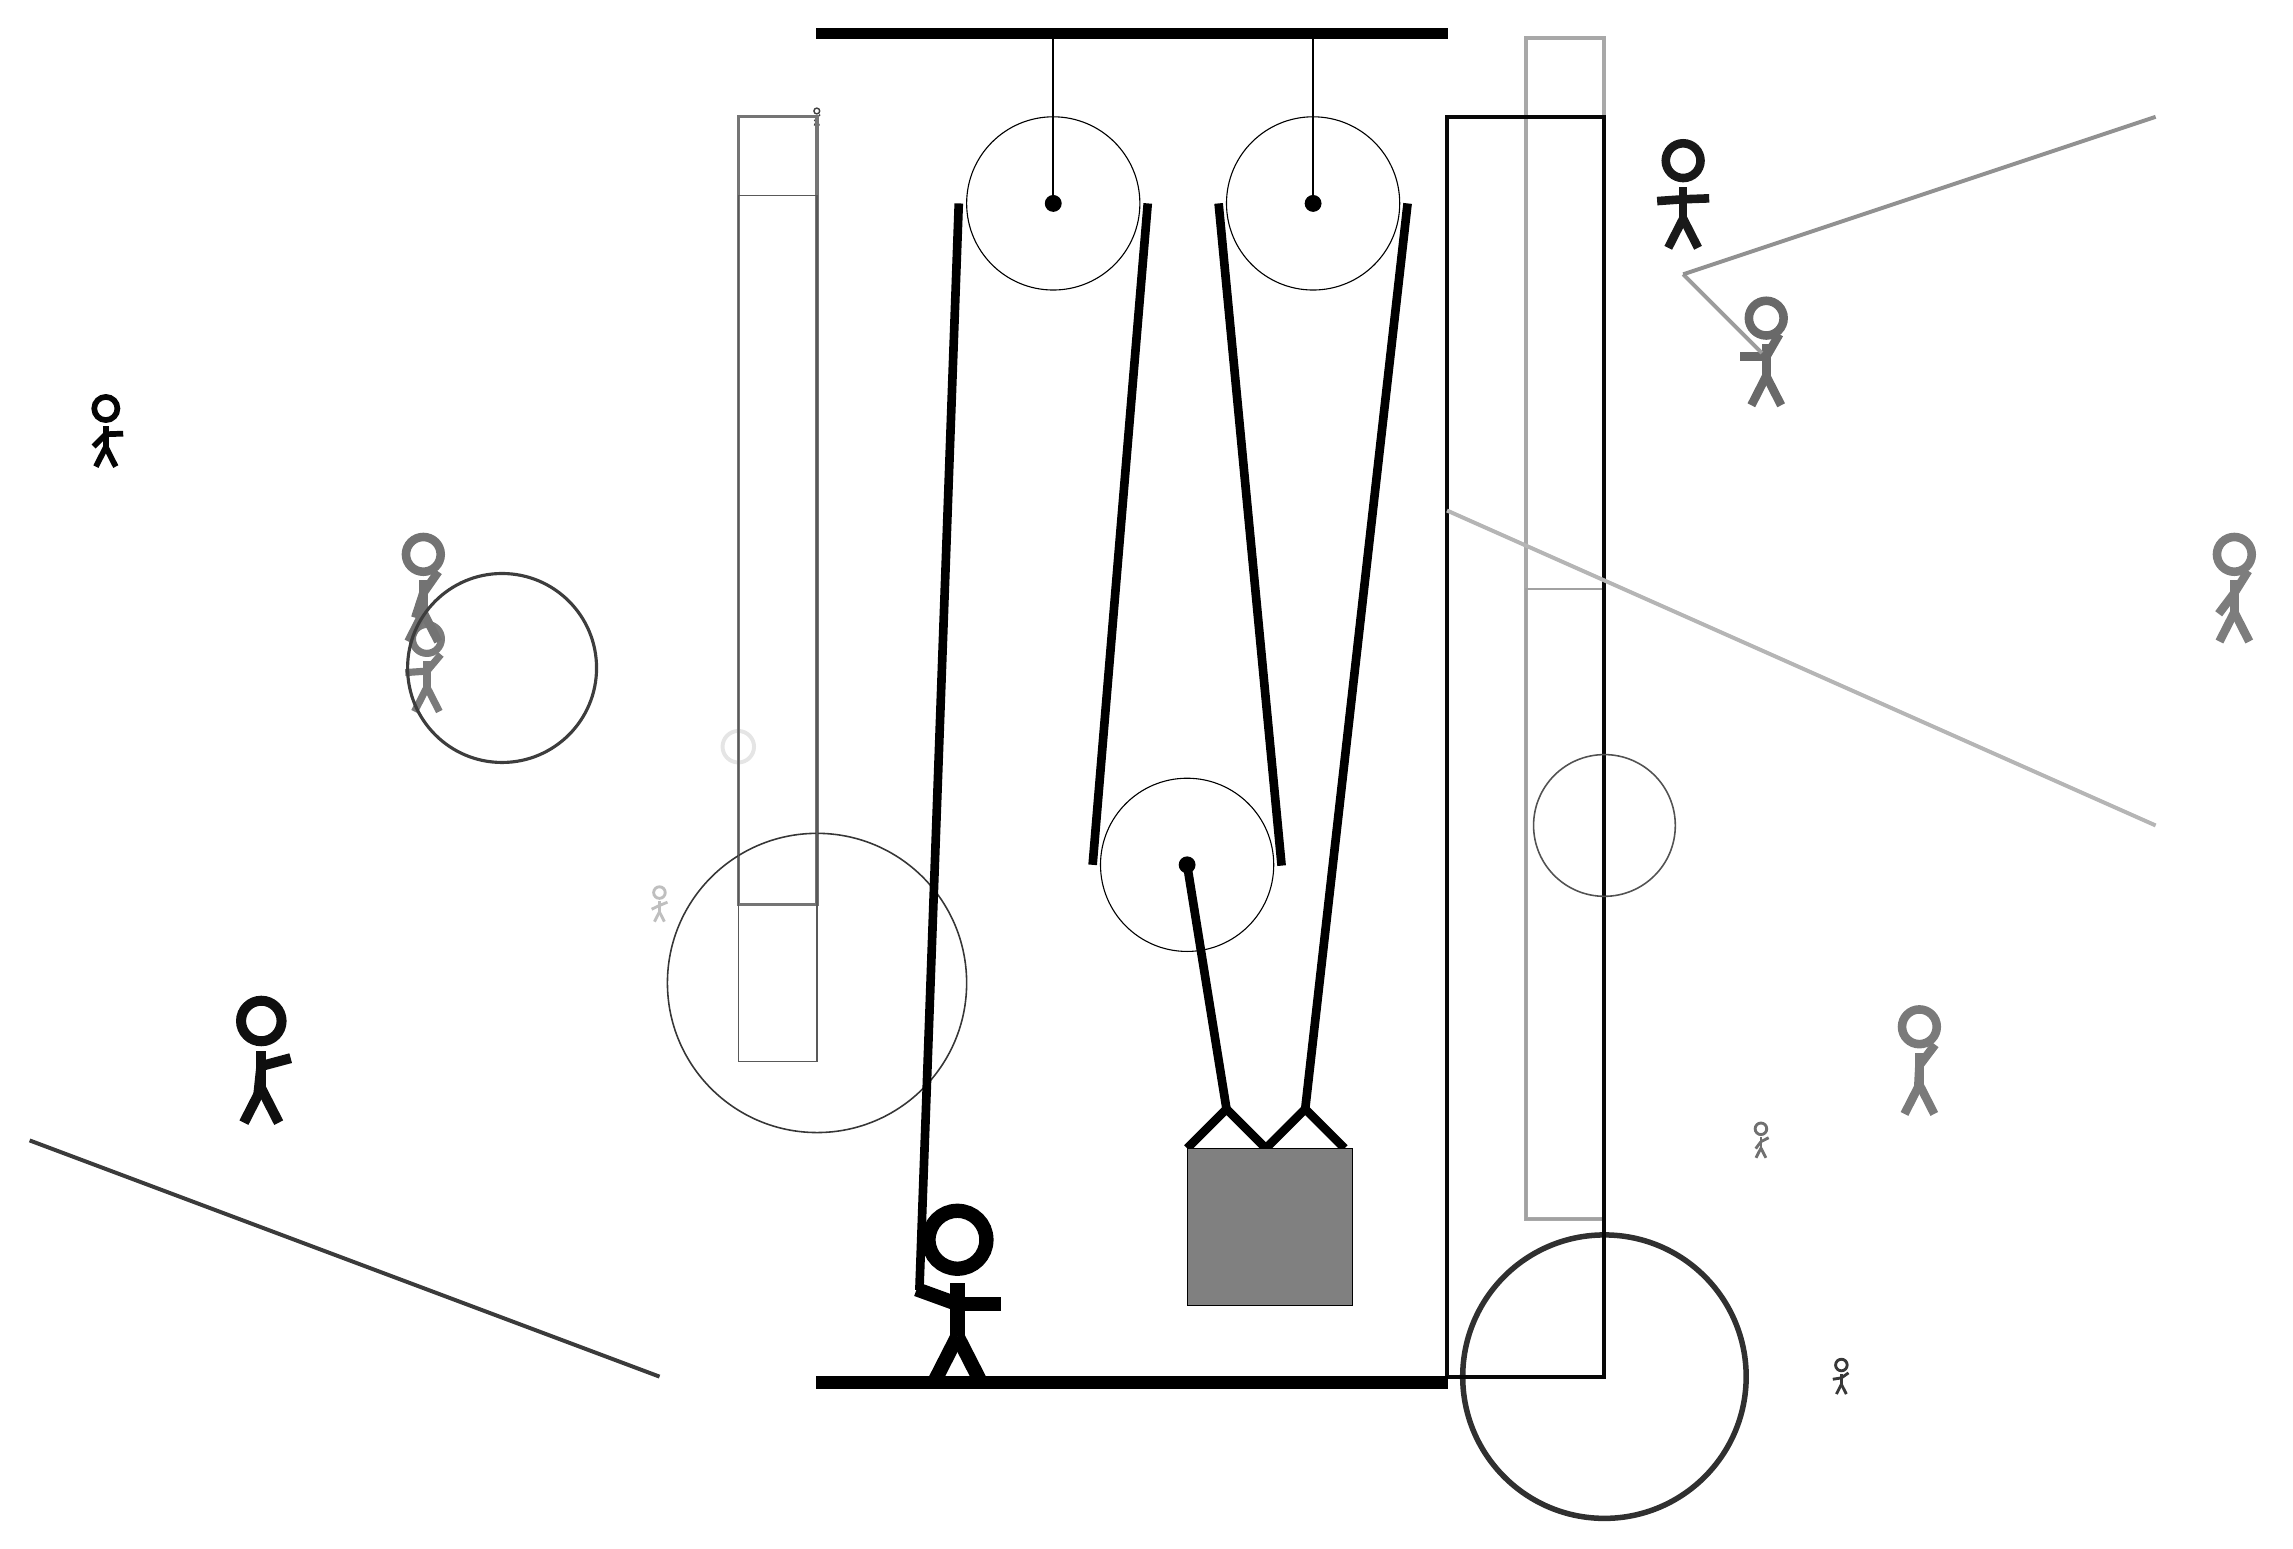
\begin{tikzpicture}
			%%%%% START %%%%%
			
			\draw[fill=black] (-2, 14) rectangle (6, 14.125);
			
			\draw (1, 11.9) circle (1.1);
			\draw[fill=black] (1, 11.9) circle (0.1);
			\draw[thick] (1, 11.9) -- (1, 14);
			
			\draw (4.3, 11.9) circle (1.1);
			\draw[fill=black] (4.3, 11.9) circle (0.1);
			\draw[thick] (4.3, 11.9) -- (4.3, 14);
			
			\node[line width=0.7mm, color=black!52] at (-7, 6) {\Strichmaxerl[5][4][50]};
			
			\node[line width=0.7mm, color=black!78] at (11, -3) {\Strichmaxerl[2][9][35]};
			\draw[line width=0.5mm, color=black!34] (8, 14) rectangle (7, -1);
			\draw[line width=0.3mm, color=black!37] (7, -1) rectangle (8, 7);
			\draw [line width=0.5mm, color=black!10](-3, 5) circle (0.2);
			
			\draw [line width=0.7mm, color=black!81](8, -3) circle (1.8);
			
			\draw[line width=0.2mm, color=black!51] (-2, 8) rectangle (-2, 8);
			\node[line width=0.7mm, color=black!98] at (-11, 9) {\Strichmaxerl[4][45][2]};
			\node[line width=0.5mm, color=black!59] at (10, 10) {\Strichmaxerl[6][0][60]};
			\node[line width=0.6mm, color=black!55] at (-7, 7) {\Strichmaxerl[6][72][55]};
			\node[line width=0.7mm, color=black!75] at (-2, 13) {\Strichmaxerl[1][58][40]};
			\draw[line width=0.5mm, color=black!39](10, 10) -- (9, 11);
			\node[line width=0.4mm, color=black!56] at (10, 0) {\Strichmaxerl[2][53][27]};
			
			\node[line width=0.5mm, color=black!51] at (16, 7) {\Strichmaxerl[6][53][58]};
			\draw[line width=0.5mm, color=black!43](9, 11) -- (15, 13);
			\node[line width=0.4mm, color=black!52] at (12, 1) {\Strichmaxerl[6][87][53]};
			\node[line width=0.2mm, color=black!25] at (-4, 3) {\Strichmaxerl[2][26][22]};
			
			\draw [line width=0.4mm, color=black!76](-6, 6) circle (1.2);
			\draw[line width=0.5mm, color=black!77](-4, -3) -- (-12, 0);
			
			\draw[line width=0.4mm, color=black!54] (-2, 13) rectangle (-3, 3);
			\draw[line width=0.5mm, color=black!97] (8, -3) rectangle (6, 13);
			\draw [line width=0.2mm, color=black!79](-2, 2) circle (1.9);
			\draw[line width=0.2mm, color=black!65] (-2, 1) rectangle (-3, 12);
			\node[line width=0.5mm, color=black!90] at (9, 12) {\Strichmaxerl[6][4][2]};
			\draw[line width=0.5mm, color=black!29](6, 8) -- (15, 4);
			
			\node[line width=0.3mm, color=black!94] at (-9, 1) {\Strichmaxerl[7][84][15]};
			\draw [line width=0.2mm, color=black!68](8, 4) circle (0.9);
			
			\draw (2.7, 3.5) circle (1.1);
			\draw[fill=black] (2.7, 3.5) circle (0.1);
			
			\draw[line width=1.1mm]  (2.7, -0.1) -- (3.2, 0.4) -- (3.7, -0.1) -- (4.2, 0.4) -- (4.7, -0.1);
			\draw[fill=black!50] (2.7, -0.1) rectangle (4.8, -2.1);
			
			\draw[line width=1.1mm](-0.7, -1.9) -- (-0.2, 11.9);
			\centerarc[line width=1.1mm](1, 11.9)(0:180:1.2000000000000002);
			\draw[line width=1.1mm](2.2, 11.9) -- (1.5, 3.5);
			\centerarc[line width=1.1mm](2.7, 3.5)(180:370:1.2000000000000002);
			\draw[line width=1.1mm] (3.9, 3.49) -- (3.1, 11.9);
			\centerarc[line width=1.1mm](4.3, 11.9)(0:180:1.2000000000000002);
			\draw[line width=1.1mm](4.2, 0.4) -- (5.5, 11.9);
			\draw[line width=1.1mm] (3.2, 0.4) -- (2.7, 3.5);
			
			\node at (-0.2, -2) {\Strichmaxerl[10][-20][0]};
			
			\draw[fill=black] (-2, -3) rectangle (6, -3.15);
			
			%%%%% END %%%%%
		\end{tikzpicture}
	\end{figure}	
\end{document}